\documentclass{article}
\usepackage{geometry}
\usepackage{spreadtab}
\usepackage{numprint}
\usepackage{caption}
\usepackage{listings}
\usepackage{spverbatim}
\usepackage{titlesec}
\usepackage{lmodern}  % for bold teletype font
\usepackage{amsmath}  % for \hookrightarrow
\usepackage{xcolor}   % for \textcolor
\usepackage{hyperref}
\usepackage{pgfplotstable}
\usepackage{pgfplots}

\pgfplotsset{width=15cm,compat=1.9}

\STautoround{2}

\geometry{legalpaper, margin=3cm}
\setlength{\parindent}{0pt}

\lstset{
  basicstyle=\ttfamily,
  columns=fullflexible,
  breaklines=true
}

\begin{document}
\title{Sherical Harmonic Representation of Earth Elevation Data - Project Report}
\author{Auguste Warmé-Janville (3800191)}
\maketitle

\section{Introduction}

\par To acknowledge which part of the sequential code needed to be parallelized, i used a GNU profiler to determine which functions were consuming the most ressources. It turned out that the QR factorization was by far the most time consuming function call. That is the part of the code we are going to try parallelize. 

\section{Parallelism strategy}

\par I chose to use the ScaLAPACK library to parallelize the QR decomposition. The matrix needs to be distributed between all the processes in a 2D block cyclic distribution for the factorization to work. Then it is sent back to the main process for the least squares problem to be minimised. All the communication between the processes are done using BLACS or MPI routines.
\par After scaling the computations to the final size, it turned out that I had to parallelize the validate function as well, since it was taking more time to validate the models than to compute them. The parallelism here is simple, each process checks one line every N line (where N is the total number of processes). For all the lines to be read, each process starts reading with an offset equal to its \verb |rank|. It is done using MPI send and receive routines.

\subsubsection*{ScaLAPACK} 
\par ScaLAPACK is a parallel version of the LAPACK library. It provides high performance linear algrebra parallel routines.

\subsubsection*{BLACS}
\par BLACS provides an linear algrebra oriented message passing interface based on MPI.

\section{Code : ScaLAPACK and BLAS routines used}

The following ScaLAPACK routines were used to make the parallel QR factorization work. The functions descriptions are extracts from the ScaLAPACK documentation.

\begin{lstlisting}[language=c]

/*
* This function computes the local number of rows or columns of a 
* block-cyclically distributed matrix contained in a process row or 
* process column, respectively, indicated by the calling sequence argument iproc.
*/
long numroc_(long* N, long* NB, long* IPROC, long *ISRCPROC, long* NPROCS );

/*
* This function computes the process row or column index of a 
* global element of a block-cyclically distributed matrix.
*/
long indxg2p_( long* INDXGLOB, long* NB, long* IPROC, long* ISRCPROC, long* NPROCS  );

/*
* The pdgemr2d routine copies the indicated matrix or submatrix 
* of A to the indicated matrix or submatrix of B. It provides a 
* truly general copy from any block cyclicly-distributed matrix 
* or submatrix to any other block cyclicly-distributed matrix or submatrix.
*/
void pdgemr2d_( long* m, long* n, double* a, long* ia, long* ja, long* desca, double* b, long* ib, long* jb, long* descb, long* ictxt);

/*
* These subroutines compute the QR factorization of a general matrix A, 
* where, in this description:
* A represents the global general submatrix Aia:ia+m-1, ja:ja+n-1 to be factored.
* For PDGEQRF, Q is an orthogonal matrix.
* For m >= n, R is an upper triangular matrix.
* If m = 0 or n = 0, no computation is performed and the subroutine returns 
* after doing some parameter checking.
*/
void pdgeqrf_(long* M, long *N, double* A, long* IA, long *JA, long* DESCA, double *TAU, double *WORK, long* LWORK, long *INFO);

/* 
* This subroutine initializes a type-1 array descriptor with error checking 
*/
void descinit_ (long *desc, const long *m, const long *n, const long *mb, const long *nb, const long *irsrc, const long *icsrc, const long *ictxt, const long *lld, long *info);

\end{lstlisting}

The BLACS routines used are the following.

\begin{lstlisting}[language=c]

extern void Cblacs_get(long icontxt, long what, long *val);
extern void Cblacs_setup(long * rank, long * nprocs);
extern void Cblacs_gridinit(long * ictx, const char * order, long nprow, long npcol);
extern void Cblacs_gridinfo(long ictx, long * nprow, long * npcol, long * myrow, long * mycol);
extern void Cblacs_gridexit( long ictx );
extern void Cblacs_exit( long doneflag );

\end{lstlisting}

\section{Implementation comments}

\subsection{Process grid}

\par For the ScaLAPACK functions to work, processes need to be arranged in a process grid \footnote{\href{https://netlib.org/scalapack/slug/node33.html\#SECTION04240000000000000000}{\textit{About process grids}}}. This is done using BLACS functions. As mentioned in the ScaLAPACK documenation, the process grid need to be a square in order to get the best perfoemance.

\subsection{Matrices 2D block cyclic distribution}

\par The matrices need to be distributed between the processes following a 2D block cyclic distribution \footnote{\href{https://netlib.org/scalapack/slug/node75.html\#SECTION04431000000000000000}{\textit{About 2D block cyclic distribution}}} for the factorization to work. It is acheived using the \verb |pdgemr2d| function. 
\par The dimensions of the process grid $p$ and $q$ are computed by the \verb |approx_sqrt(int a, int *p, int *q)| function which computes the integers $p$ and $q$ ($p \leq q$) such that $a = p \times q$ and the length of the interval $[p, q]$ is minimal. If $a$ is a square, $p = q = \sqrt a$. The size of the blocks is determined by the global variable \verb |BLOCK_SIZE|. The ScaLAPACK user guide recommends a block size of 64 \footnote{\href{https://netlib.org/scalapack/slug/node106.html\#SECTION04511000000000000000}{\textit{About ScaLAPACK performance}}}. 

\subsection{Points selection}

\par In order to reduce the size of the matrices we're working on, we need to skip some datapoints on the hi and ultra sets. Thus, I modified the function that reads the points from the file and added a command line option to the \textit{model} program : \verb |--spacing|. It is quite straightforward. If a spacing of N points is specified, the program will sample only $1$ point every $N$ points from the dataset. The \verb |--npoint| option remains unchanged. It must be set to the max number of points the set contains for the program to iterate over all of them. As a result, the value of the variable \verb |npoint| from the main function, which represents the number of rows of the matrix (which is different from the command line option) is equal to $npoints/spacing$. 
    
\subsection{Running the code on multiple g5k nodes : HOW2}
\par The main focus here is that ScaLAPACK needs to be installed on each session on every available node before running the \verb |model| function. These are the steps to follow :

\begin{itemize}
    \item Reserve some nodes from the same cluster
    \item Install scalapack on all the nodes via ssh : run the \verb |install_scalapack.sh| script
    \item Compile the code (\verb |make|)
    \item Run it 
    \begin{itemize}
        \item model : \begin{spverbatim} mpirun -n <core_count> -machinefile $OAR_NODEFILE ./model --data <filename> --model <model> --npoint <npoints> --lmax <lmax> --spacing <spacing> \end{spverbatim}
        \item validate : \begin{spverbatim} mpirun -n <core_count> -machinefile $OAR_NODEFILE ./validate --data <filename> --model <model> --lmax <lmax> \end{spverbatim} 
    \end{itemize}
    
\end{itemize}

\section{Speedup, Scalability}
\subsection{Large Matrix : 2.1Go size, 4:1 ratio}

\par These results were acheived using 4 nodes (64 cores) from the grisou cluster. We're measuring the performance of the implementation on large matrices. We're also comparing the performance depending on the block size.

\subsubsection*{Model, block\_size=8}
\begin{center}
\begin{spreadtab}{{tabular}{|c|c|c|c|c|}}
    \hline
    @Processor count & @Computing time (in seconds) & @Speedup & @Efficiency & @GFLOPS \\
    \hline
    1   &   1592.0     & b2 / b2    & c2   / a2  & 2.7  \\
    8   &   104.25     & b2 / b3    & c3   / a3  & 41   \\
    16  &   63.95      & b2 / b4    & c4   / a4  & 66   \\
    24  &   46.25      & b2 / b5    & c5   / a5  & 91   \\
    32  &   37.33      & b2 / b6    & c6   / a6  & 114  \\
    40  &   32.34      & b2 / b7    & c7   / a7  & 131  \\
    48  &   28.61      & b2 / b8    & c8   / a8  & 149  \\
    56  &   26.32      & b2 / b9    & c9   / a9  & 162  \\
    64  &   24.43      & b2 / b10   & c10  / a10 & 174  \\
    \hline
\end{spreadtab}
\captionof{table}{\textit{Model : npoint = 32400, nvar = 8100, hi dataset, spacing = 200, block size =  8}}
\end{center}

\subsubsection*{Model, block\_size=64}

\begin{center}
\begin{spreadtab}{{tabular}{|c|c|c|c|c|}}
    \hline
    @Processor count & @Computing time (in seconds) & @Speedup & @Efficiency & @GFLOPS \\
    \hline
    1   &   1574.0     & b2 / b2    & c2   / a2  & 2.7  \\
    8   &   62.78      & b2 / b3    & c3   / a3  & 68    \\
    16  &   37.17      & b2 / b4    & c4   / a4  & 114   \\
    24  &   29.25      & b2 / b5    & c5   / a5  & 145   \\
    32  &   25.29      & b2 / b6    & c6   / a6  & 168  \\
    40  &   22.42      & b2 / b7    & c7   / a7  & 189  \\
    48  &   20.38      & b2 / b8    & c8   / a8  & 208  \\
    56  &   20.19      & b2 / b9    & c9   / a9  & 210  \\
    64  &   19.07      & b2 / b10   & c10  / a10 & 223  \\
    \hline
\end{spreadtab}
\captionof{table}{\textit{Model : npoint = 32400, nvar = 8100, hi dataset, spacing = 200, block size =  64}}
\end{center}

\subsubsection*{Validate}

\begin{center}
    \begin{spreadtab}{{tabular}{|c|c|c|c|}}
        \hline
        @Processor count & @Computing time (in seconds) & @Speedup & @Efficiency \\
        \hline
        1   &   707    & b2 / b2  & c2  / a2  \\
        8   &   98.9   & b2 / b3  & c3  / a3  \\
        16  &   59.9   & b2 / b4  & c4  / a4  \\
        24  &   38.3   & b2 / b5  & c5  / a5  \\
        32  &   30.1   & b2 / b6  & c6  / a6  \\
        40  &   23.5   & b2 / b7  & c7  / a7  \\
        48  &   18.8   & b2 / b8  & c8  / a8  \\
        56  &   16.8   & b2 / b9  & c9  / a9  \\
        64  &   14.6   & b2 / b10 & c10 / a10 \\
        \hline
\end{spreadtab}
\captionof{table}{\textit{Validate : lmax = 89, hi dataset}}
\end{center}

\par As specified in the ScaLAPACK user manual, the efficiency of this computation is greater with a block size of 64 compared to a block size of 8. Indeed, as the block size increases, the number of communication routines called decreases, thus the global computation runtime also decreases.
\par As well as the speedup induced by the pallarelization, the parralel ScaLAPACK version is overall more efficient than the sequential program, as the speedup is superior to 1 for any core count greater than one on the \verb |model| function analysis. This makes ScaLAPACK a good choice for big linear algebra computations (what a surpise !).

\subsection{Comparison between different matrices sizes}

\par I measured the speedup of the model function for different matrices dimensions (4:1 ratio) on different sets, and plotted the results. The core count varies from 8 to 64 by increments of 8. The legend follows the formatting \textit{dataset/lmax/spacing/matrix\_size}. The block size is equal to 64. \\

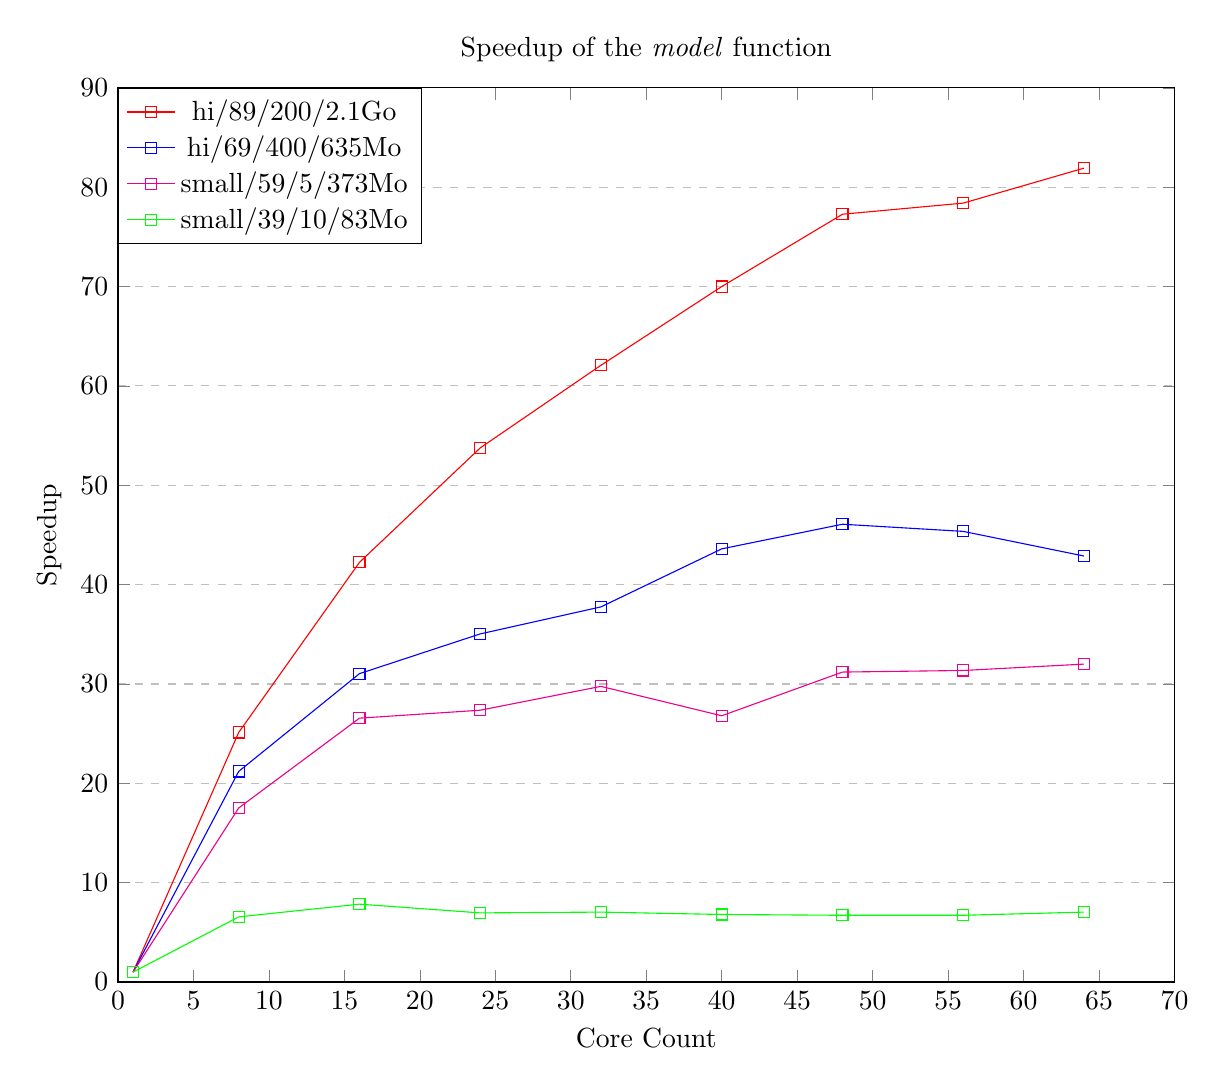
\begin{tikzpicture}
\begin{axis}[
    title={Speedup of the \textit{model} function},
    xlabel={Core Count},
    ylabel={Speedup},
    xmin=0, xmax=70,
    ymin=0, ymax=90,
    legend pos=north west,
    ymajorgrids=true,
    grid style=dashed,
    legend entries={hi/89/200/2.1Go, hi/69/400/635Mo, small/59/5/373Mo, small/39/10/83Mo},
    legend style={at={(0,1)},anchor=north west},
]

\addplot[
    color=red,
    mark=square,
    ]
    coordinates {
        (1, 1)
        (8, 3.14 * 8)
        (16, 2.64 * 16)
        (24, 2.24 * 24)
        (32, 1.94 * 32)
        (40, 1.75 * 40)
        (48, 1.61 * 48)
        (56, 1.40 * 56)
        (64, 1.28 * 64)
    };

\addplot[
    color=blue,
    mark=square,
    ]
    coordinates {
        (1, 1)
        (8, 2.65 * 8)
        (16, 1.94 * 16)
        (24, 1.46 * 24)
        (32, 1.18 * 32)
        (40, 1.09 * 40)
        (48, 0.96 * 48)
        (56, 0.81 * 56)
        (64, 0.67 * 64)
    };


\addplot[
    color=magenta,
    mark=square,
    ]
    coordinates {
        (1, 1)
        (8, 2.19 * 8)
        (16, 1.66 * 16)
        (24, 1.14 * 24)
        (32, 0.93 * 32)
        (40, 0.67 * 40)
        (48, 0.65 * 48)
        (56, 0.56 * 56)
        (64, 0.50 * 64)
    };

\addplot[
    color=green,
    mark=square,
    ]
    coordinates {
        (1, 1)
        (8, 0.82 * 8)
        (16, 0.49 * 16)
        (24, 0.29 * 24)
        (32, 0.22 * 32)
        (40, 0.17 * 40)
        (48, 0.14 * 48)
        (56, 0.12 * 56)
        (64, 0.11 * 64)
    };
    
\end{axis}
\end{tikzpicture} \\

As the size of the matrix decreases, the speedup incuded by the parallelization also decreases. To a reduced scale of time, the inter-processes communications takes a not negligible amount of time. If the parallel \verb |model| program is run on too small matrices, the performance gain becomes null. Therefore, it is not especially a good idea to run the parallel program on small matrices, it is just going to consume more energy, if it doesn't simply makes the sequential program slower. An idea to improve the sequential performance would the be to use LAPACK functions that are designed for these kinds of computations.

\subsection{Conclusion}

Parallelizing the sequential code using ScaLAPACK turns out to be very efficient, as long as the matrices on which the computation is done are big enough. However, this implementation can not be scaled to matrices with sizes greater than 16 Go (see the section about Bugs and Crashes). 

\section{Best model}

\par The best model I computed is contained in the file \verb |model_ul_129_2200.txt|. The parameters are : 

\begin{itemize}
    \item dataset = ultra
    \item lmax = 129
    \item npoints = 233280000
    \item spacing = 2200
\end{itemize}

Running this program produces a matrix which dimensions are 106036 x 16900. It requires 14.3 GB RAM.  
\par The \verb |validate| function returns : 

\begin{itemize}
    \item Average error = 229.034 meters
    \item Max error = 6781.6 meters
    \item Standard Deviation = 382.026
\end{itemize}

Since it looks like working with matrices with size greater than 16Go makes the program crash, I could not push the computation any further. 

\section{Bugs/Crashes}
    
\par On large matrices, the code often crashes for certain values of lmax (\verb |xxmr2d:out of memory|). This has to do with the 2D block cyclic distribution function. As well, on very large matrices (16 Go size), the program crashes (\verb |segfault, address not mapped|). This is caused by the ScaLAPACK prebuilt libary which uses 4 bytes integers, thus the max size for a double precision float matrix is 16 Go. A potential fix would be to rebuild the library with 8 bytes integers, but I did not had time to do it.

\end{document}
